\documentclass[letterpaper,10pt]{article}

%\setlength{\parindent}{0in}
%\usepackage{fullpage} 
\usepackage{amsmath}
\usepackage{amssymb}
\usepackage{enumerate}
\usepackage{graphicx}
\usepackage[table]{xcolor}
\usepackage{dcolumn}
\oddsidemargin 0.0in
\textwidth 6.5in
\newcolumntype{.}{D{.}{.}{-1}}
\newcommand*{\myalign}[2]{\multicolumn{1}{#1}{#2}}

%opening
\title{Final Exam}
\author{Steve Mazza}
%\date{December 9, 2011}

\begin{document}
\maketitle

\begin{description}
\item[Question 1:]
Given the differential equation $\dfrac{d^4y}{dx^4}+\dfrac{d^2y}{dx^2}=0\equiv y''''+Ay''$ derive the equivalent system of first-order ordinary differential equations.  This is a fourth order differential equation.  What order is the system of equations?  Is the system linear or nonlinear?  What does such a system of first-order ordinary differential equations represent?

%TODO: Answer question. (mazzas) Fri Jun 13 18:20:42 2014
Based on slide deck 2, slide 7, I assume this is a linear system since it can be broken up into parts.

\item[Question 2:]
The Maxwell-Bloch equations are a sophisticated model for a laser and describe the dynamics of the electric field $E$, the mean polarization of the atoms $P$, and the population inversion $D$:
\begin{align*}
\dot{E} &= (P-E) \\
\dot{P} &= \gamma_1(ED-P) \\
\dot{D} &= \gamma_2(\lambda+1-D-EP)
\end{align*}
where $\gamma_1$ and $\gamma_2$ are decay rates of the atomic polarization and population inversion, respectively, and $\lambda$ is a pumping energy parameter.  The parameter $\lambda$ may be positive, negative, or zero; all other parameters are positive.  In the simplest case, $P$ and $D$ relax rapidly to steady values, and hence may be eliminated as follows.
\begin{enumerate}
\item Assuming $\dot{D}\approx 0$\ $\dot{P}\approx 0$, express $P$ and $D$ in terms of $E$, and thereby derive a first-order equation for the evolution of $E$.
\item Find all the fixed points of $E$.
\item Draw the bifurcation diagram of $E^*$ versus $\lambda$.  Distinguish between stable and unstable branches.
\end{enumerate}

Slide deck 4, slides 31 \& 39 talks about fixed points.

This is Strogatz problem 3.3.2, page 82.

%TODO: Answer question. (mazzas) Fri Jun 13 18:21:02 2014

\item[Question 3:]
What is this an example of?  What features are represented?
\begin{center}
  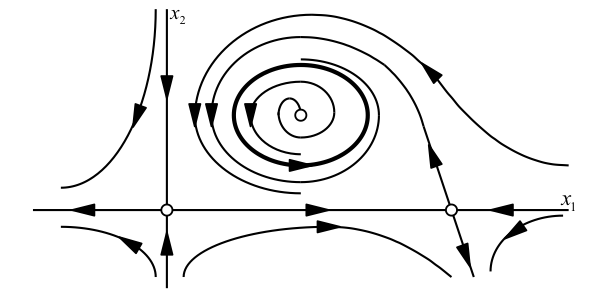
\includegraphics[scale=0.65]{images/phaseportrait.png}
\end{center}

slide deck 3, slide 4: the exact example!!!

See Strogatz, page 146.

A phase portrait is a qualitative picture of the behavior of a system in phase space.  Typically it shows fixed points, the stability of fixed points, closed orbits, and trajectories near the fixed points and closed orbits.  The phase portrait below is illustrative only and does not represent a specific system.

%TODO: Answer question. (mazzas) Fri Jun 13 18:21:20 2014

\item[Question 4:]
For the Lorenz equations
\begin{align*}
\dot{x} &= \sigma(y-x) \\
\dot{y} &= rx-y-xz \\
\dot{z} &= xy-bz
\end{align*}
with $\sigma=10, r=28$, and $b=2.66666$, and initial condition $x=1.0+\delta, y=1.0$, and $z=10$, determine how long it takes the absolute error between the ``true $x$ solution'' $(\delta=0)$ to grow from $\delta$ to 0.1. Calculate for $\delta$ values of 0.01, $10^{-4}, 10^{-6}, 10^{-8}$, and $10^{-10}$.  What does this tell you about the predictability versus measurement error?  Can you estimate the Liapunov exponent? (Strogatz, 366)

Slide deck 4, slide 45 talks about Liapunov exponents.

This looks just like Strogatz, page 339.
%TODO: Answer question. (mazzas) Fri Jun 13 18:21:38 2014

\item[Question 5:]
Consider the iterated map given by
\[x_{n+1} = \left\{
  \begin{array}{lr}
    rx_n &  0\le x_n \le 0.5 \\
    f(1-x_n) &  0.5\le x_n \le 1
  \end{array}
\right.
\]
where $0<r<2$.  What properties do you expect to see in the orbit diagram?  Is there any condition that might cause different behavior?  The Liapunov exponent is $\lambda=\mbox{ln\ }r$. (Strogatz, 366)  What does this tell you about the behavior?

%TODO: Answer question. (mazzas) Fri Jun 13 18:21:59 2014

\item[Question 6:]
  In your own words and using no more than one paragraph, describe the difference between complex and complicated systems.  That is, in your own opinion what distinguishes the two?

Week 1 slide deck, slide 46.

Axelrod, page 15.

Complexity vs. Complicated
\begin{itemize}
  \item Complexity is often differentiated from complicated.
  \item A complicated or complex system must have a large number of parts.  One or two parts cannot be complicated.  (Note: if a part can be decomposed into other parts, then it is a system not a part).
  \item A system is complicated if it collapses (fails to function) if any small subset of non-redundant parts is eliminated.
  \item A system is complex if it continues to function (possibly in a degraded fashion) if any small subset of parts is removed.
  \item A watch has many diverse elements that are connected and interdependent.  The watch is complicated if it stops working when a gear is removed.  The watch is complex if it continues to function due to some form of functional (vice physical) redundancy when that gear is removed.
\end{itemize}

%TODO: Answer question. (mazzas) Fri Jun 13 18:22:14 2014

\item[Question 7:]
How are fractals and complexity related?

See Mitchell, page 103.  The answer is, ``though fractal dimension.''

%TODO: Answer question. (mazzas) Fri Jun 13 18:22:33 2014

\item[Question 8:]
Define what an adaptive agent-based model is and briefly describe its characteristics.

Slide deck 1, slide 84.
%TODO: Answer question. (mazzas) Fri Jun 13 18:22:45 2014

Agent based models.
\begin{itemize}
  \item Ideas drive the development of tools (quarks drive accelerators) or tools may drive the development of ideas (microscopes drive microbiology).
  \item Agent-based models are computer models that permit the exploration of complex systems in more detail.
  \item Agent-based models consist of entities of various types (the agents) endowed with limited memory and cognitive ability that are embedded in a network (connected to other agents) and whose behaviors are interdependent (usually locally).
  \item Agents follow rules.  The rules may be simple and fixed or complicated and adaptive.
  \item Adaptive agents follow metarules, which are rules about how rules can be changed.
  \item Agents often take discrete actions such as changing location, switching strategy (cooperation vs. defection), or joining or exiting a particular activity.
  \item Rules are often threshold-based, that is, rules in which the agent’s behavior remains the same until some threshold is met.
  \item Threshold effects can cause positive (more of the same) or negative (less of the same) feedbacks.
  \item Agent-based systems often exhibit complex, emergent behavior.
\end{itemize}

\item[Question 9:]
In an engineering system consisting of various parts and mechanisms, what kinds of diversity are most applicable to determining complexity?  How might that diversity be measured?

Slide deck 1, slides 58-62, focusing on slide 62.
%TODO: Answer question. (mazzas) Fri Jun 13 18:22:57 2014

Complexity (from slide 62)
\begin{itemize}
  \item Variation within a type seldom results in complexity
  \item Differences between types is often associated with complexity
  \item Diversity in composition is often associated with complexity
\end{itemize}

Five kinds of diversity measures (from slide 59)
\begin{itemize}
  \item Variation measures
  \item Entropy measures
  \item Distance measures
  \item Attribute measures
  \item Disjoint population measures
\end{itemize}
Also see slides 60 \& 61

\item[Question 10:]
What approaches are likely to [be] part of any attempt to harness complexity in an inherently complex system?

Also see slide deck 1, slides 104 \& 105.

In ``Harnessing Complexity,'' Axelrod \& Cohen present a framework for harnessing complexity, which the refer to as the Complex Adaptive Systems approach.  They describe various techniques of variation, interaction, and selection that the user of a system can leverage to affect or sway the outcome of a complex adaptive system.

The following ideas are summarized from the section titled, ``What a User of the Framework Can Do,'' in the Conclusion of their book.

\begin{description}
  \item[Variation] \ \\
    \begin{itemize}
      \item Arrange organizational routines to generate a good balance between exploration and exploitation.
      \item Link processes that generate extreme variation to processes that select with few mistakes in the attribution of credit.
    \end{itemize}
  \item[Interaction] \ \\
    \begin{itemize}
      \item Build networks of reciprocal interaction that foster trust and cooperation.
      \item Assess strategies in light of how their consequences can spread.
      \item Promote effective neighborhoods.
      \item Do not sow large failures when reaping small efficiencies.
    \end{itemize}
  \item[Selection] \ \\
    \begin{itemize}
      \item Use social activity to promote the growth and spread of valued criteria.
      \item Look for shorter-term, finer-grained measures of success that can usefully stand in for longer-run, broader goals.
    \end{itemize}
\end{description}

Detailed explanations of these approaches can be found on pages 155 -- 158.

\end{description}
\end{document}
